\subsection{Component View}
This section aims at illustrating the various components that make up the \app system. In the following, UML Component diagrams are employed to illustrate the logical software elements that collaborate in order to achieve the goals set for the system to be developed.

Since the structure of components of the \app system wouldn't fit into a single diagram, multiple representations are supplied to make the document as clear as possible and avoid cluttering. 
The decisions regarding how to divide the diagrams of the Component View have been taken based on the idea of grouping together components that frequently interact with each other. 
It is important to mention that although the explanation makes use of separated graphics, the system is a single one and the elements represented here in different diagrams will be part of the same system and will take part in the overall functioning of the platform together.

\subsubsection{RESTful APIs component diagram}
\begin{minipage}{\linewidth}
One of the first characteristics that have been mentioned in the introductory section about \app is that microservices expose RESTful APIs in order to receive and respond to commands, expose data and collaborate with one another. This view aims at describing from a high perspective the ways microservices exploit these APIs to work.

\vspace*{1.5cm}
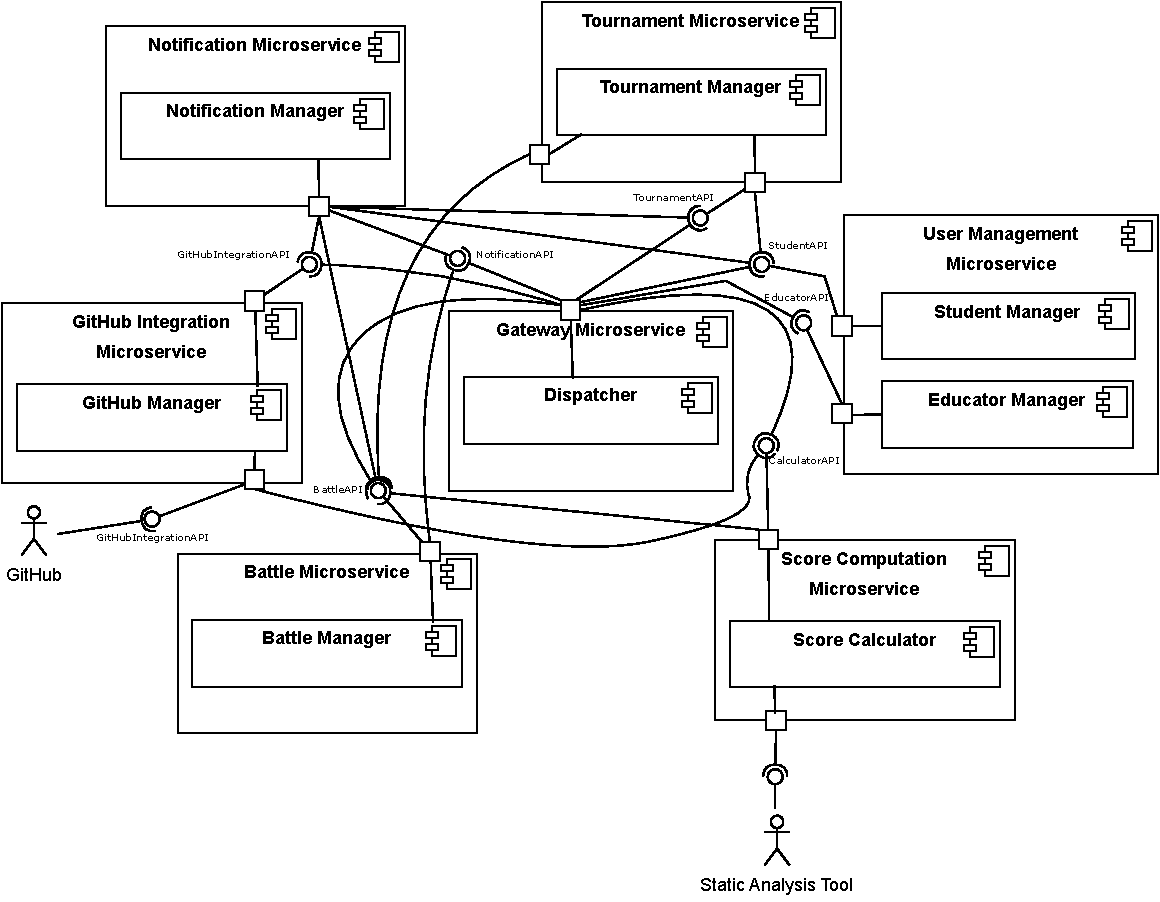
\includegraphics[width=\linewidth]{1Component_REST_API}

\end{minipage}

Let's break down the main ideas that the diagram tries to convey.
This UML component diagram is employed in order to show the RESTful APIs that are offered by each microservice in the system. These APIs provide specific computations on data related to the service offered by the microservice in question. For instance, the Tournament Microservice will expose an API that works on the tournaments data inside the shared database and exposes relevant information on tournaments.

The gateway is the entry point for all users’ requests. The Dispatcher component inside the Gateway is responsible for delivering the users' requests to the correct microservices that will have to handle them. This is why the Dispatcher "uses" all the APIs exposed by the other microservices. 

For some kinds of computations, the various microservices that compose \app may also exploit each other through their RESTful APIs. In this diagram, these interactions are shown. 
For instance:
\begin{itemize}
	\item The Notification Manager needs to query the Tournament manager and the Battle manager every time it has to retrieve the list of students subscribed to a tournament or to a battle (in order to deliver the notification to a specific set of students).
	\item The Notification Manager has to query the Student Manager when the list of all students of CodeKataBattle is needed (for example to notify all students of a new tournament available on the platform).
	\item The Notification Manager requires access to the data handled by the GitHub Manager in order to retrieve the link to the remote repository of a battle and compose the notification for all students subscribed to that battle (when the registration deadline of the battle passes).
	\item The GitHub manager component uses the CalculatorAPI in order to pass the downloaded source code of a new student solution to the Score Calculator component that will in turn automatically compute the score to assign to it.
	\item The Score Calculator must exploit the BattleAPI in order to request an update on the battle ranking every time a new score is available.
	\item The Tournament Manager requires access to the Student Manager data in order to assign badges when the tournament is closed.
	\item The Battle Manager leverages the NotificationAPI in order to produce individual notifications when a student invites another student to join a battle together as a team.
\end{itemize}

This diagram has to be read and interpreted also accounting for the event-driven paradigm that is adopted in the project. Some of the interactions and flows of events inside the system happen in an asynchronous manner with an event-driven approach that is further described in the following views. That's why some interactions, that might seem missing here are actually handled in an asynchronous way to increase the performance of the overall system.

The last important point to make about this diagram is related to the "Manager" components inside the various microservices. These components internally implement a Model-View-Controller pattern to provide their services. The following representation shows a component diagram that only focuses on the internals of the "Manager" component for a generic microservice:

\vspace{1cm}
\begin{center}
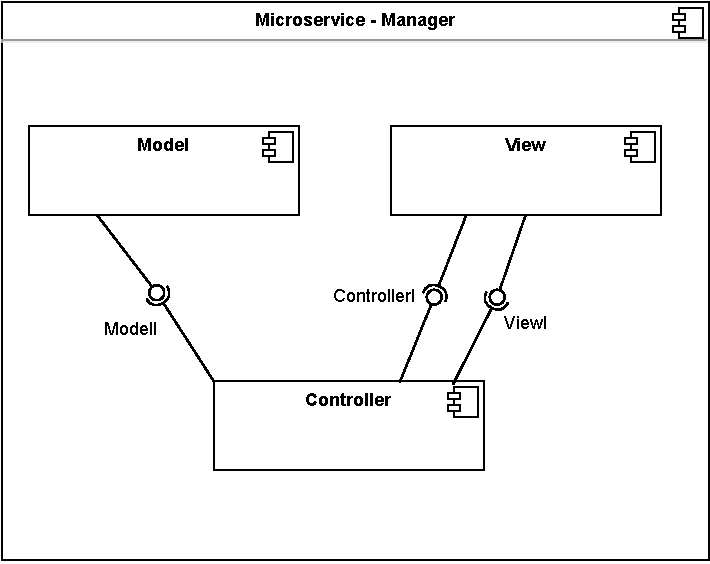
\includegraphics[width=0.6\linewidth]{1.1Component_MVC_Pattern}
\end{center}

The Model component is responsible for organizing and managing data. Each microservice in the \app system is specific for a portion of the data domain. For instance, the Tournament Microservice only focuses on managing and providing information on tournaments. Therefore, each Model component inside the Manager components take care of maintaining consistent data with the DBMS, accessing the DBMS when needed and so on.

The View is the component offering the user interface. Since different microservices focus on different types of information in the \app ecosystem, the several user interfaces are spread across the microservices and managed through the View components.

The Controller is the "bridge" between the Model and the View. This component is responsible for:
\begin{itemize}
	\item Receiving the requests from the View component when the user interacts with the user interface. 
	\item Performing the correct computation based on those requests.
	\item Manipulating data through the Model, propagating the users' requests to the data layer.
	\item Updating the View if the computation resulted in some changes of the user interface.
\end{itemize}

In the following of the document, the Manager component will be used in a more general sense to capture the behavior and functionality of all this internal architecture.


\subsubsection{Service Discovery component diagram}

\begin{minipage}{\linewidth}
	
	This very simple component diagram shows an important service that is offered by the Gateway microservice to allow all microservices to locate each other and therefore collaborate. This service is called "Service Discovery" and it consists in maintaining a register (inside the Gateway microservice) of active microservices. 
	
	In this way:
	\begin{itemize}
		\item A new microservice brought up can register itself in order to be localized by the other microservices.
		\item All microservices can contact other active microservices in the system to advance some requests.
	\end{itemize}
	
	Here's the diagram:
	
	\vspace{2cm}
	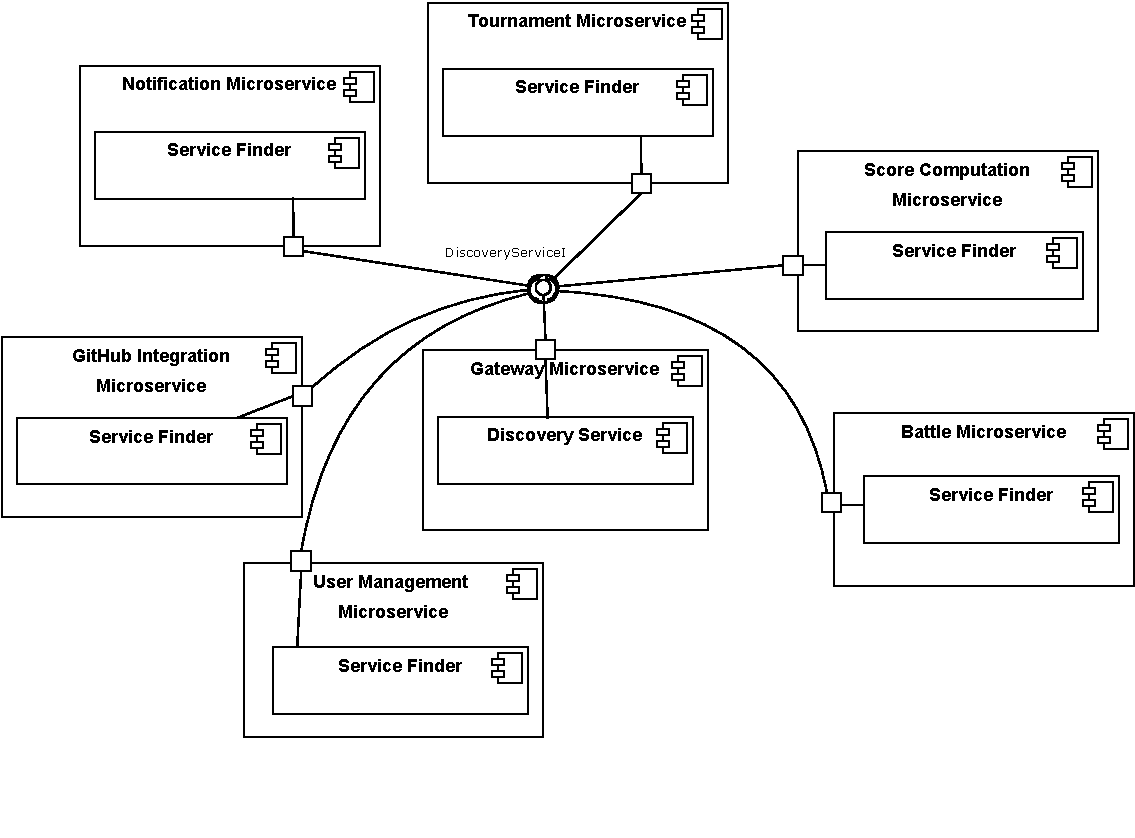
\includegraphics[width=\linewidth]{2Component_ServiceDiscovery}
	
\end{minipage}

	The interpretation is quite simple. The Gateway Microservice contains a component called Discovery Service, which is the software component that implements the logic to offer the discovery service. The Discovery Service component exposes an API (DiscoveryServiceI), that can be used by all other microservices in order to locate each other. 

\subsubsection{Event-driven pattern components}
\begin{minipage}{\linewidth}
	This section illustrates all the components that are needed in the system in order to implement an asynchronous, event-driven communication between microservices. This design choice has been taken in order to lighten up the system in specific interactions between microservices that would otherwise require a computationally expensive synchronous communication.
	
	The following diagram shows the major components that help achieve an event-driven architecture:
	
	\vspace{2cm}
	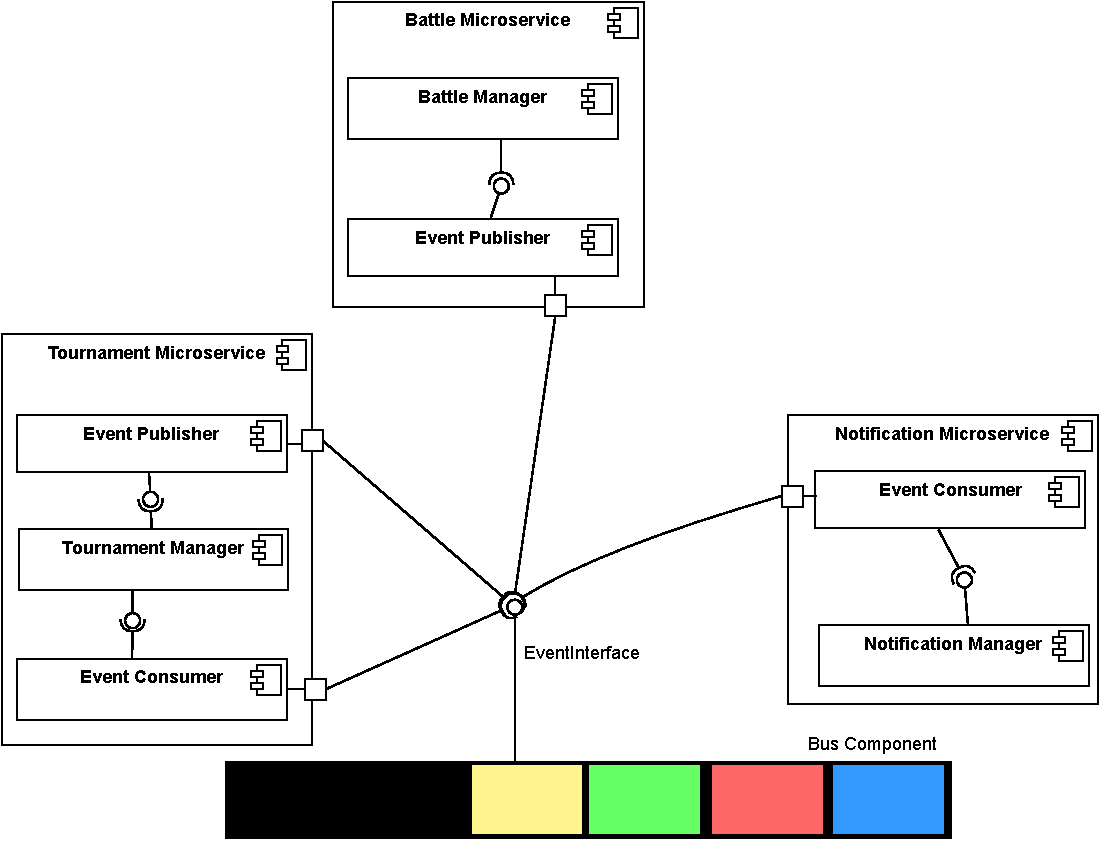
\includegraphics[width=\linewidth]{3Component_EventDriven}
	
	\vspace{2cm}
	
\end{minipage}

The most important element is the Bus component, which can be thought of as a queue of messages or events. Microservices in the \app system can either produce events (i.e. push events on the queue) or consume events (i.e. read events on the queue) and take actions accordingly.

It is important to mention that this representation is purposely general and not tied up with any specific software product, framework or implementation. The concrete way in which this design is achieved is left to the implementation of the product.

From the diagram, it is possible to see that only some microservices are illustrated, which are the only one exploiting this mechanism to communicate and interact. 
Inside these microservices, there is an Event Publisher component if the microservice has to be able to publish events on the Bus, and there might be an Event Consumer component in case the microservice has to be able to read from the Bus the events that are queued.

The Tournament Microservice, for instance, has both the Event Publisher component and the Event Consumer component. Indeed, the Tournament Microservice has to publish an event every time a new tournament is created or closed. At the same time, the tournament has to be able to read from the bus when a battle is finished, to take actions accordingly. 

The Battle Microservice only publishes events when the battle is created and terminates.

The GitHub Integration Microservice publishes a new event every time the GitHub repository for a battle is created, since a notification to all the students subscribed to that battle has to be fabricated.

The Notification Microservice is the one always listening to upcoming events in order to fabricate the correct notifications for the users of the \app platform.




\subsubsection{Data layer access component diagram}
\begin{minipage}{\linewidth}
	This diagram proposes a convenient view to see how the access is performed by the various microservices on the shared data layer (shared DBMS).
	
	\vspace{2cm}
	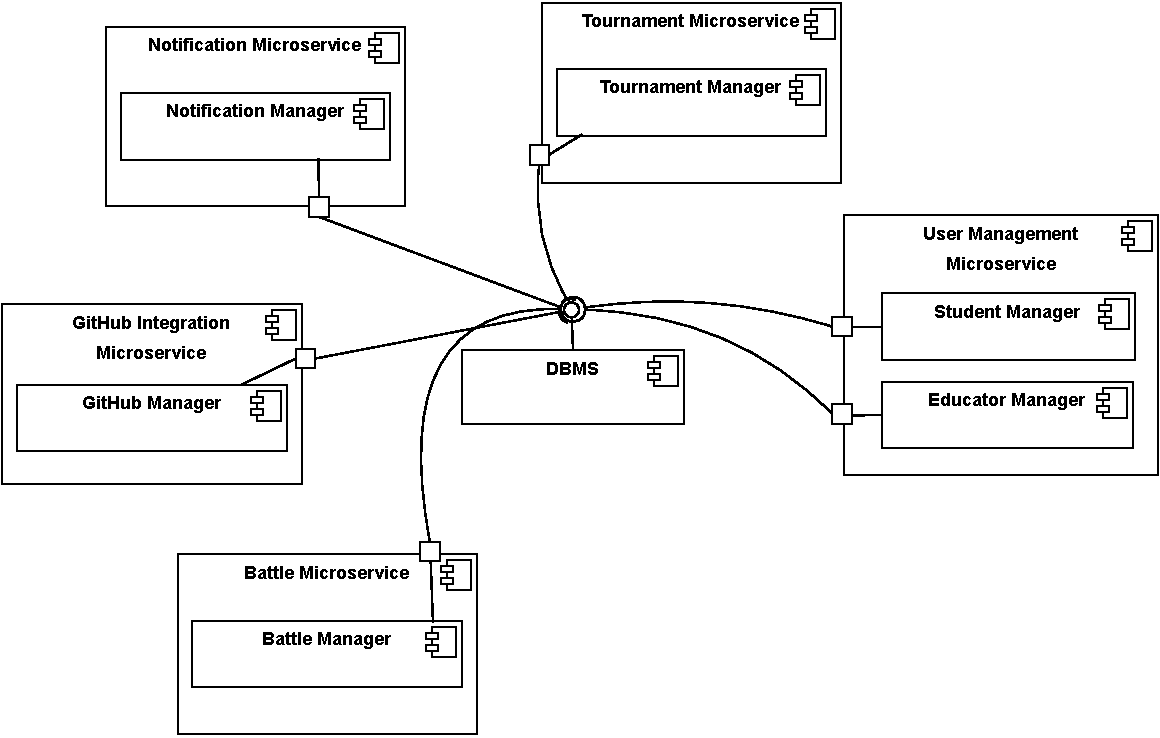
\includegraphics[width=\linewidth]{4Component_DataAccess}
	
	\vspace{2cm}
	
	The DBMS exposes an interface that is employed by all microservices to work with the persistent data stored in the DBMS.
	
	Looking at every microservice individually, it is possible to notice that they all are equipped with a "Manager" component, which is responsible for manipulating and accessing data.
	
	Every microservice of the \app application is responsible for a different section of the data domain. For instance, the Tournament microservice only works on the data stored in the shared DBMS that is related to tournaments and offers to the other microservices all the relevant information about tournaments that might be needed.
	

\end{minipage}

\subsubsection{User interfaces component diagram}
\begin{minipage}{\linewidth}
	This diagram proposes a convenient view of the system for what concerns user interfaces. The design choices that have been taken in the \app system as concerns the user interfaces can be summed up in this way:
	
	\begin{itemize}
		\item The different interfaces that are offered to the user are not gathered in a single component, but they are scattered across the various microservices. This decision is due to the fact that different UIs offer different views on the data of the application. Therefore, some microservices (working on a specific section of the data domain) might be more suitable for providing a specific user interface than others.
		\item All the times a user interface is offered to the user, the Gateway Microservice handles the transmission of data, standing in between the user and the access to the internal microservice. Therefore, all the UIs content passes by the Gateway before reaching the client user.
	\end{itemize}
	
	This diagram tries to illustrate the two points of the above list, by representing a View component inside each microservice that is responsible for building and offering specific user interfaces when required. 
	The Gateway microservice intercepts the user's requests and when a new UI is needed, it contacts the correct microservice that will supply it.
	It has to be mentioned the fact that this UML diagram is not a standard one, in the sense that the interfaces exposed by the components in this view are not sets of methods but UIs. Nevertheless it is intended as a beneficial illustration to show part of the MVC pattern (with the View components inside the microservices) and the distribution of UIs in the system.
	
	\begin{center}
	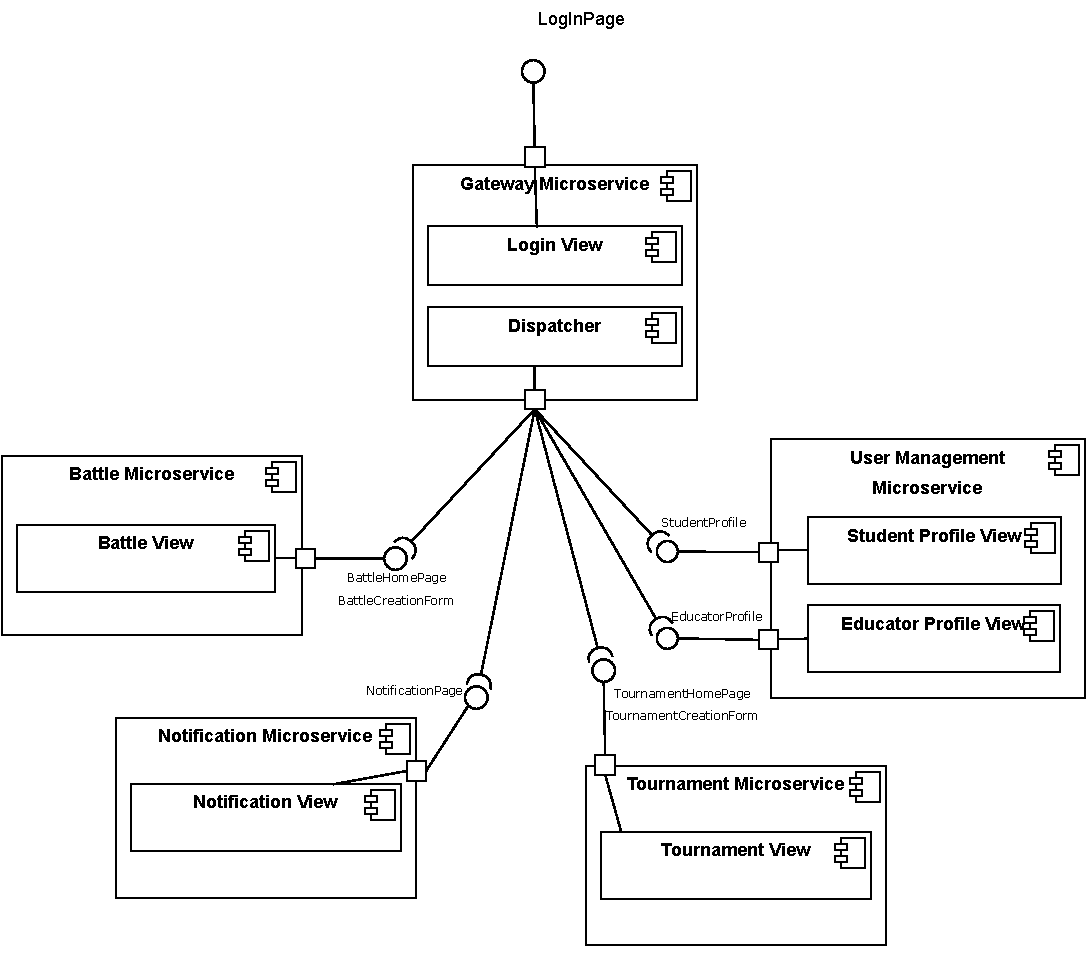
\includegraphics[width=0.8\linewidth]{5Component_ViewsUI}
	\end{center}
	
	
\end{minipage}